% Where the record of an individual's work exists, and where it stops.
% Monochrome with a single accent; serif to match the body text.
\documentclass[tikz,border=3mm]{standalone}
\usepackage{tikz}
\usetikzlibrary{arrows.meta,positioning,calc,backgrounds,fit}

\definecolor{ink}{HTML}{1A1A1A}
\definecolor{accent}{HTML}{8C1D18}
\definecolor{mute}{HTML}{9A9A9A}

\begin{document}
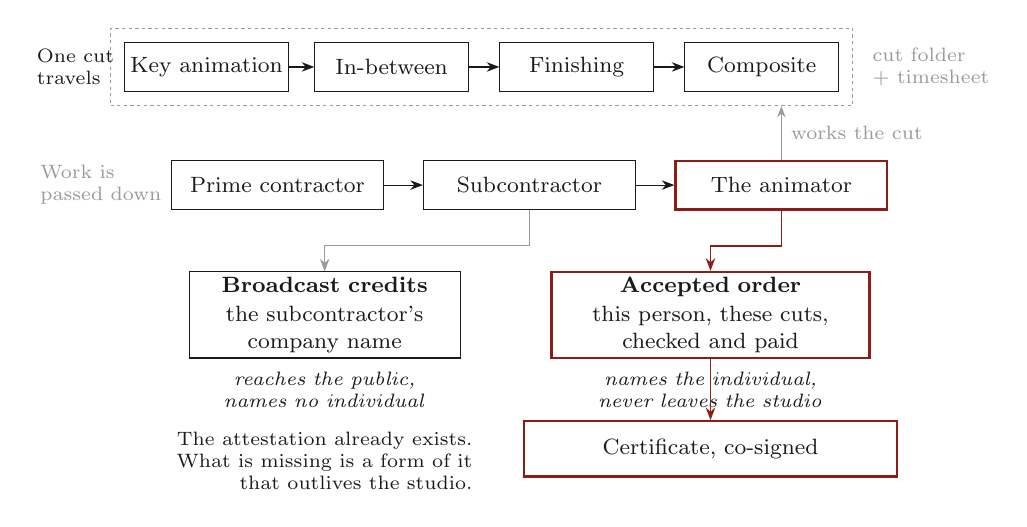
\begin{tikzpicture}[
  font=\footnotesize\rmfamily, ink,
  tier/.style={draw=ink, line width=0.4pt, minimum height=0.62cm,
               text width=2.55cm, align=center, inner sep=2pt},
  stage/.style={draw=ink, line width=0.4pt, minimum height=0.62cm,
                minimum width=1.95cm, align=center, inner sep=2pt},
  flow/.style={-{Stealth[length=1.6mm]}, draw=ink, line width=0.4pt},
  faint/.style={draw=mute, line width=0.35pt},
  note/.style={font=\scriptsize\rmfamily, text=ink, align=left},
  hilite/.style={draw=accent, line width=0.8pt},
]

% ---- the cut travelling through stages -------------------------------------
\node[stage] (key)   at (0,0)      {Key animation};
\node[stage] (inb)   at (2.35,0)   {In-between};
\node[stage] (fin)   at (4.70,0)   {Finishing};
\node[stage] (comp)  at (7.05,0)   {Composite};

\draw[flow] (key) -- (inb);
\draw[flow] (inb) -- (fin);
\draw[flow] (fin) -- (comp);

\node[note, anchor=east] at (-1.05,0) {One cut\\travels};

% the physical carrier
\begin{scope}[on background layer]
  \node[draw=mute, line width=0.35pt, dash pattern=on 1.2pt off 1.2pt,
        fit=(key)(comp), inner sep=5pt] (folder) {};
\end{scope}
\node[note, anchor=west, text=mute] at ($(folder.east)+(0.12,0)$)
  {cut folder\\+ timesheet};

% ---- who actually did it ----------------------------------------------------
\node[tier] (prime)  at (0.9,-1.5)  {Prime contractor};
\node[tier] (sub)    at (4.1,-1.5)  {Subcontractor};
\node[tier, hilite] (person) at (7.3,-1.5) {The animator};

\draw[flow] (prime) -- (sub);
\draw[flow] (sub) -- (person);
\node[note, anchor=east, text=mute] at (-0.45,-1.5) {Work is\\passed down};

\draw[faint, -{Stealth[length=1.4mm]}] (person.north) -- (folder.south -| person.north)
  node[midway, right, font=\scriptsize\rmfamily, text=mute] {works the cut};

% ---- the two records that result -------------------------------------------
\node[tier, text width=3.3cm, minimum height=0.95cm] (credits) at (1.5,-3.15)
  {\textbf{Broadcast credits}\\[1pt] the subcontractor's\\company name};
\node[tier, text width=3.9cm, minimum height=0.95cm, hilite] (order) at (6.4,-3.15)
  {\textbf{Accepted order}\\[1pt] this person, these cuts,\\checked and paid};

\draw[flow, draw=mute] (sub.south) -- ++(0,-0.45) -| (credits.north);
\draw[flow, draw=accent] (person.south) -- ++(0,-0.45) -| (order.north);

\node[note, anchor=north, text width=3.3cm, align=center] at (1.5,-3.75)
  {\textit{reaches the public,\\names no individual}};
\node[note, anchor=north, text width=4.1cm, align=center] at (6.4,-3.75)
  {\textit{names the individual,\\never leaves the studio}};

% ---- what the certificate does ----------------------------------------------
\node[tier, text width=4.6cm, minimum height=0.7cm, hilite] (sbt) at (6.4,-4.85)
  {Certificate, co-signed};
\draw[flow, draw=accent] (order.south) -- ++(0,-0.55) -- (sbt.north);

\node[note, anchor=east, text width=4.4cm] at (3.5,-5.0)
  {\raggedleft The attestation already exists.\\What is missing is a form of it\\that outlives the studio.\par};

\end{tikzpicture}
\end{document}
